\documentclass[a4paper,10pt, twoside]{article}
\usepackage[margin=1.4in]{geometry}
\usepackage[swedish]{babel}
\usepackage[utf8]{inputenc}
\usepackage{titlesec}
\usepackage{titling}
\usepackage{todonotes}



\setlength{\parskip}{1em}
\setlength{\parindent}{0pt}
\titlespacing{\section}{0pt}{\parskip}{-\parskip}
\titlespacing{\subsection}{0pt}{\parskip}{-\parskip}
\titlespacing{\subsubsection}{0pt}{\parskip}{-\parskip}
\titlespacing{\part}{0pt}{\parskip}{-\parskip}

\usepackage{adjustbox}
\usepackage[backend=bibtex,sorting=none]{biblatex}
\addbibresource{bib-arkitektur.bib}
\externaldocument[krav-]{../Kravspec/kravspec}

\begin{document}
\def\ftitle{Arkitekturdokument}
\def\fversion{1.1}
\begin{titlepage} % Suppresses displaying the page number on the title page and the subsequent page counts as page 1
	\newcommand{\HRule}{\rule{\linewidth}{0.5mm}} % Defines a new command for horizontal lines, change thickness here

	\center % Centre everything on the page

	%------------------------------------------------
	%	Headings
	%------------------------------------------------

	\textsc{\LARGE Linköpings universitet \\ \vspace{0.2em} Institutionen för datavetenskap }\\[2cm]

    \large\today

    \vspace{1cm}


	%------------------------------------------------
	%	Title
	%------------------------------------------------

	\HRule\\[0.4cm]

	{\huge\bfseries Schemaläggningsstöd för  kirurgi \vspace{.1em} \\ \ftitle }\\[0.4cm] % Title of your document

	\HRule\\[1cm]

	%------------------------------------------------
	%	Author(s)
	%------------------------------------------------

	\begin{minipage}{0.7\textwidth}
			\large
            \emph{Version: \fversion}
            \vspace{1em}

            \textbf{\\Adam Andersson, Niclas Byrsten, \\Björn Hvass, Henrik Lindström, \\Martin Persson, Christoffer Sjöbergsson, \\Tor Utterborn}


            \vspace{1em}

            Handledare: Jonas Wallgren

            Examinator: Kristian Sandahl
	\end{minipage}
	~

	%------------------------------------------------
	%	Logo
	%------------------------------------------------

	%\vfill\vfill
	%
\includegraphics[width=0.2\textwidth]{../Templates/Aeon}\\[1cm] % Include a department/university logo - this will require the graphicx package

	%----------------------------------------------------------------------------------------

	\vfill % Push the date up 1/4 of the remaining page

\end{titlepage}


\section*{\begin{center}Projektidentitet\end{center}}
    \vspace{-2.5em}
    \begin{center}
        \begin{tabular}{|c c c|}
        \hline
        Namn & Roll & E-post \\
        \hline
        Adam Andersson& Teamleader & adam.e.a.andersson@gmail.com\\
        \hline
        Niclas Byrsten & Testansvarig & nicby889@student.liu.se\\
        \hline
        Björn Hvass & Konfigurationsansvarig & bjorn.hvass@gmail.com\\
        \hline
        Henrik Lindström & Utvecklingsledare & henli070@student.liu.se\\
        \hline
        Martin Persson & Arkitekturansvarig & marpe902@liu.student.se\\
        \hline
        Christoffer Sjöbersson & Analysansvarig & chrsj812@liu.student.se\\
        \hline
        Tor Utterborn & Dokument- \& Kvalitetsansvarig & tor.utterborn@gmail.com\\
        \hline
        \end{tabular}
    \end{center}

    \begin{center}
        \small
        \textbf{Kund}\\Region Östergötland, 581 91 Linköping.

        \textbf{Kontaktperson hos kund}\\
        Gunnar Nordqvist, IT-arkitekt, 010-1030698, Gunnar.Nordqvist@regionostergotland.se\\
        Erik Sundvall, Informationsarkitekt, 010-1036252, Erik.Sundvall@regionostergotland.se
    \end{center}

\vspace{9em}



\section*{\begin{center}Dokumentationshistorik\end{center}}
\begin{center}
 \begin{tabular}{|c c c c |}
 \hline
 Datum & händelse & iteration & version\\
 \hline
 2018-02-10 & Dokument skapas & 1 &  0.1\\
 \hline
  2018-02-19 & Konvertering till \textbf{\LaTeX} & 1 &  0.2\\
 \hline
   2018-02-19 & Version 1.0 färdigställd & 1 &  1.0\\
 \hline
 	2018-04-20 & Systemskiss uppdaterad & 2 & 1.1
\end{tabular}
\clearpage
\end{center}
\tableofcontents
\clearpage
\section{Inledning}
\label{sec:Inledning}
Här presenteras en översikt av vad dokumentet innehåller och hur systemet är uppbyggt.

\subsection{Syfte}
Arkitekturdokumentet ger en översikt av schemaläggningssystemets arkitektur. I dokumentet presenteras arkitekturen samt en översiktlig beskrivning av systemet och dess funktionalitet. Här finns även en genomgång av de arki1tektuellt signifikanta beslut som fattats och varför de fattats. Dokumentet är tänkt att användas av både beställare och projektgrupp för att få en inblick i vilka arkitektoniska beslut som fattats och varför.

\subsection{Ordlista}
Här förklaras tekniska termer och förkortningar.
\begin{itemize}
  \item MVC   (Model-view-controller) Ett designmönster för gränssnitt.
  \item JSON  (JavaScript Object Notation) Filtyp för att överföra data som objekt i JavaScript.
  \item AJAX  (Asynchronous JavaScript And XML) En metod för att hantera kommunikation mellan klient och server. Kommer i detta system implementeras med JSON-filer.
\end{itemize}

\subsection{Översiktlig systembeskrivning}
Det schemaläggningssystem som ska utvecklas kommer användas på operationsavdelningen i ett sjukhus av sjukhuspersonal för planering av operationer. Systemet ska klara av att utifrån en lista med beslutade operationer ge användaren förslag på operationstider inom operationens tidsgräns då rätt lokal och resurser finns tillgängliga. För tider då lokal finns att tillgå men resurser saknas ska systemet visa vilka resurser som saknas. Användaren ska utifrån detta kunna välja en passande tid och boka in operationen. Besluten ska innehålla relevanta data om patient och operationstyp, och det ska för varje beslut framgå om beslutet behandlats eller inte. Ifall patienten behöver flera ingrepp ska användaren kunna se detta och kunna slå samman ingreppen till en operation vid behov.

Operationer ska kunna avbokas och frigöras från schemat. Det ska finnas en schemaöversikt med en filterfunktion som visar när vilka resurser är lediga eller upptagna. Det ska finnas en tidslinje över operationen som visar när operationsprocessens olika stadier börjar. Det ska gå att logga vilken användare som bokat vad. All information ska lagras i en central databas. Från databasen ska informationen hämtas ned till användardatorer via en server. Systemet ska visas på en skärm och användaren interagerar med det med hjälp av tangentbord och mus.


\subsection{Mål och filosofi}
Målet med utvecklingen av systemet är att ta fram en prototyp för ett schemaläggningsverktyg som kan användas som underlag för att få en bild av vilken funktionalitet som ett verkligt schemaläggningsverktyg behöver ha. Då systemet inte kommer tas i egentlig drift prioriteras användbarhet och designlösningar framför prestanda. Ett väl designat användargränssnitt är huvudmålet med projektet.

\subsection{Beroenden}
Utveckling av systemet kommer ske med Angular, vilket får konsekvenser för arkitekturen. Databasen kommer implementeras med MySQL och kommer kommunicera med klienten via ett API som översätter datan till JSON-filer.

\section{Arkitektoniskt signifikanta krav}
Här listas några krav som är relevanta för arkitekturen. Kraven är hämtade ur projektets kravspecifikation\cite{kravspec}.

\begin{tabular}{|c|p{6cm}|c|}
  \hline
  Krav & Kravbeskrivning & Betydelse \\
  \hline
  \ref{krav-subsec:Hognivasprakkrav} & Klienten ska använda sig av Angular och TypeScript. & Begränsar hur klienten kan implementeras.
  \\
  \hline
  \ref{krav-subsec:EG-Mjukvarugranssnitt} & Klienten ska kunna köras på Internet Explorer 11. & Måste anpassas efter en äldre webbläsare.
  \\
  \hline
  \ref{krav-subsec:Generella krav} & Det ska gå att logga in och det ska \hyphenation{finnas}finnas en databas. & Måste ha en klient-server arkitektur.
  \\
  \hline
\end{tabular}

\subsection{Tilltänkta användare}
Systemet skall främst användas av erfarna operationsplanerare som tidigare arbetat med schemaläggning. Även annan vårdpersonal kan komma att använda systemet.

\section{Designbeslut och motivering}
Här beskrivs designbeslut som fattats eller förkastats och motiveringar av dessa.

\subsection{Model-view-controller}
För att enkelt kunna arbeta parallellt på systemets olika delar togs beslutet att använda designmönstret Model-view-controller.

Då gruppen kände att MVC var ett lämpligt mönster för webutveckling och passade väl in med valet av Angular som utvecklingsplattform och den struktur på front-end delen av arkitekturen som detta kom att resultera i så betraktades inga andra alternativ.

\subsection{Angular}
Till webbklienten beslutades att ramverkat Angular ska användas. Detta för att underlätta strukturen och designen av gränssnitt.
Ett alternativ till Angular som diskuterades var React. Att Angular föredrogs berodde inte på några direkt tekniska anledningar utan baserades på önskan från kunden Region Östergötland.

\subsection{Node.js}
På serversidan beslutades att Node.js kommer att användas. Det fanns ett par motiveringar till detta. Eftersom Angular, som kräver Node.js, redan var beslutat att användas kommer alla projektmedlemmar redan behöva Node.js installerat. Sedan använder Node.js JavaScript vilket gruppen även kommer använda till webbklienten vilket betyder att inget extra programmeringsspråk måste läras in. Till sist kan Node.js vara värd för en webbsida utan att extra mjukvara behöver laddas ner.

Eftersom Node.js har allt som önskas till projektet har andra alternativ inte undersökts.

\subsection{MySQL med JSON-API}
Som databashanterare valdes MySQL. Ett alternativ som också diskuterades var MongoDB som är en objekt-baserad hanterare\cite{mongodbintro} till skillnad från MySQL som är tabell-baserad.

Anledningen att MySQL föredrogs var eftersom Region Östergötland tillhandahåller testdata till systemet i tabell-form.

Det API som sköter kommunikation mellan klient och server skall översätta testdatan från tabellformat till JSON-filer, eftersom JSON-filer är enklare att arbeta med än tabelldata i JavaScript.

\section{Designmönster}
Här beskrivs några använda designmönster.

\subsection{Model-view-controller}
Designmönstret MVC för användargränssnitt möjliggör separation av hur gränssnittets data representeras internt sättet datorn visas upp för användare. Designmönstret delar upp gränssnittet i tre delar, Model, View och Controller.\cite{mvc} Delarna beskrivs nedan:
\begin{itemize}
  \item Model innehåller gränssnittets data och logik för att manipulera datan.
  \item View presenterar data från Model för användaren.
  \item Controller hanterar kommunikation mellan användare och Model.
\end{itemize}

\subsubsection{MVC och Angular}

Eftersom att webbapplikationen kommer att bygga på ramverket Angular blir användandet av designmönstret Model-view-controller naturligt. Angular uppmuntrar en struktur där gränssnitt och applikationslogik är uppdelade. Förutom detta kommer även funktionerna för datahämtning att vara separata från applikationslogiken. Mer om strukturen på webbklienten går att läsa i sektion \ref{sec:webbklient}.

\clearpage
\section{Systemskiss}
\label{sec:Systemskiss}
Här visas och beskrivs en översiktlig skiss av schemaläggningssystemet där det framgår vilken funktionalitet som ska köras var i systemet. \\
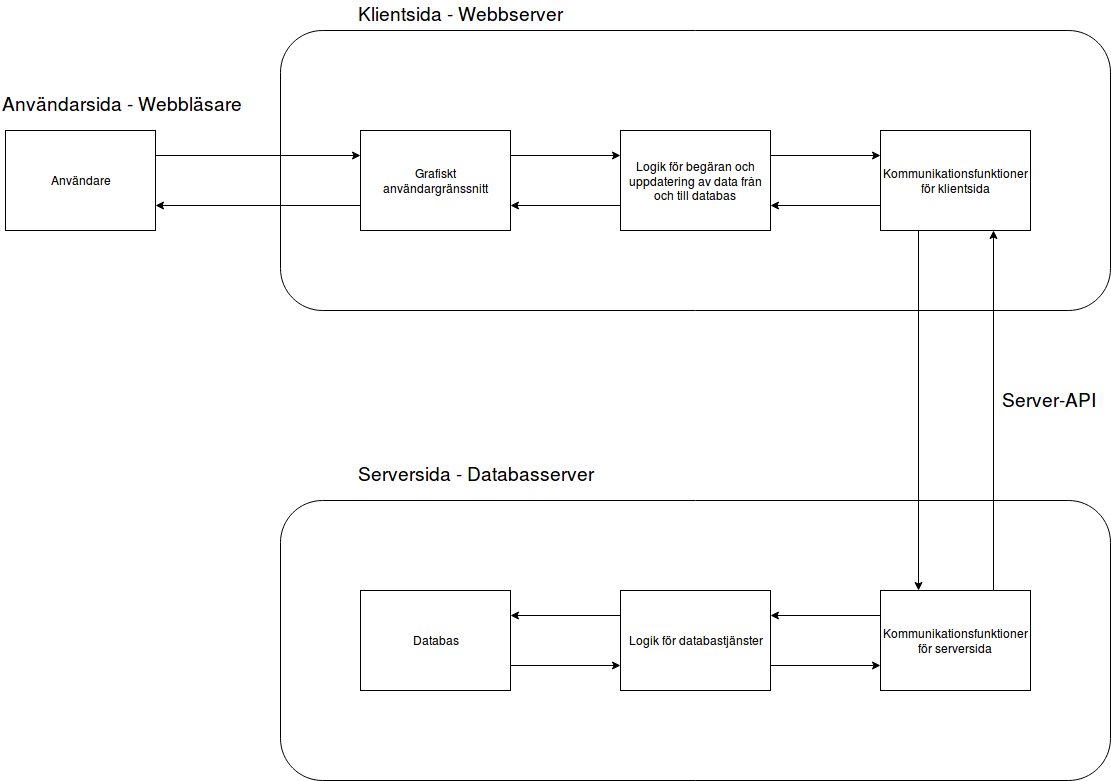
\includegraphics[width=\textwidth,height=.7\textheight]{Systemskiss.png}\\
Figur 2: Systemskiss

Systemet som beskrivs översiktligt i Figur 2 är uppdelat i två delar, en webbklient och en webbserver.
\section{Webbklient}
\label{sec:webbklient}
Webbklienten körs i en webbläsare och kommer att byggas på webbapplikationsramverket Angular. Dess struktur kommer att består av tre delar, en gränssnittsdel, en applikationslogikdel och en kommunikationsdel. I klientdelen i Figur 2 visas hur delarna hänger ihop och beror på varandra.

\subsection{Angular}
Denna sektion behandlar de delar ur Angulars arkitekturguide \cite{angularguide} som kommer att vara relevanta i projektet.

En Angular-applikation är uppbyggd av en eller flera moduler som i sin tur består av komponenter och tjänster.
\subsubsection{Komponenter}
\label{sec:komponent}
Angularkomponenter används för att dela upp gränssnittet i olika återanvändbara delar. Varje komponent ansvarar för en egen del av gränssnittet och består av dels en HTML-mall som beskriver dess utseende och dels en TypeScript-klass som hanterar allt det dynamiska med komponenten.

Komponentens mall definieras med hjälp av en något utökad HTML-syntax. All vanlig HTML förutom dess script-taggar får användas. Det tillkommer även en Angular-specifik syntax som tillåter mallen att anpassa sitt utseende beroende på klassens tillstånd.
\subsubsection{Tjänster}
Tjänster i Angular är klasser, skrivna i TypeScript, som tillhandahåller funktioner och logik som krävs av modulens komponenter eller andra tjänster. Typiskt ska de ha ett smalt och väldefinierat syfte.

\subsection{Gränssnittsdel}
Gränssnittsdelen har hand om allt som har med användarupplevelse och grafik i applikationen. Den kommer uteslutande att bestå av Angluar-komponenter som beskrivna i sektion \ref{sec:komponent}.

Varje komponent ska ha ett väldefinierat syfte och såvida den inte är trivial bör den vara uppdelad i andra mindre komponenter. Komponenternas klasser ska endast innehålla den logik som krävs för visning och interaktion med användaren. Alla andra funktioner som krävs men som inte direkt har med användarupplevelsen att göra ska istället hanteras av tjänster i applikationslogikdelen.

\subsection{Applikationslogikdel}
Denna del har som uppgift att tillhandahålla all applikationsfunktionalitet som krävs av komponenterna i gränssnittsdelen. I denna del ska det endast finnas Angular-tjänster vilka ska ha smala och väldefinierade ansvarsområden.

\subsection{Kommunikationsdel}
Kommunikationsdelen ska sköta all kommunikation med webbservern som krävs av applikationslogiken. Den ska endast bestå av Angular-tjänster.

\section{Webbserver}
\label{sec:webbserver}
Webbservern har två huvuduppgifter. Den första är att vara värd åt webbklienten så att den är tillgänglig för flera olika användare och datorer. Den andra är att hantera en databas för att lagra information om bland annat operationsbeslut, konton, resurser med mera. Detta innefattar att utföra och svara på databasförfrågningar som kommer från klienten.

Webbservern kommer att använda sig av Node.js och ska struktureras i två delar. En för kommunikation och en för databaslogik, se serverdelen i Figur 2. MySQL kommer att användas som databashanterare.

\subsection{Logikdel}
I logikdelen ligger all funktionalitet för hantering av databasen. Allt som krävs för att kunna utföra och svara på webbklientens databasförfrågningar ska finnas.

\subsection{Kommunikationdel}
Kommunikationsdelen i webbservern hanterar alla förfrågningar som kommer från användare. Den ska leverera webbklienten till användare och svara på förfrågningar från webbklienten med hjälp av funktionerna i logikdelen.

\section{Dynamiskt beteende}
Kommunikation mellan klienten och servern kommer att ske för att uppdatera den dynamiska information som klienten behöver. Detta är bland annat all indata till systemet som beskrivs i bilaga \ref{krav-sec:Ingaende data till systemet} i kravspecifikationen\cite{kravspec}, men även data om gjorda bokningar osv.

Denna information kommer att begäras av klienten vid behov vilket görs genom AJAX-begäran till servern som hittar den efterfrågade informationen och svarar med JSON.

\clearpage
\printbibliography
\end{document}
